\documentclass[letterpaper, 12pt]{article}
\usepackage[letterpaper, top=2.5cm, bottom=2.5cm, left=3cm, right=3cm]{geometry} %margenes
\usepackage[utf8]{inputenc} %manejo de caracteres especiales
\usepackage[spanish]{babel} %manejo de encabezados de inglés a español
\usepackage{fancyhdr} %formato de los encabezados de página
\usepackage{ragged2e} %alineado real justficado
\usepackage{graphicx} %manejo de imagenes
\usepackage{amsmath} %manejo de notación matemática
\usepackage{mathtools} %manejo de notación matemática
\usepackage{blindtext} %texto de relleno
\usepackage{amssymb}
\usepackage[backend=biber]{biblatex}\addbibresource{bibliografia.bib}
\usepackage[titles]{tocloft} %manejo de elementos para el índice
\usepackage{float} %manejo de centrado para figuras
\usepackage{algorithm2e} %manejo de algoritmos
\usepackage{tikz} %lineas entre matrices
\usetikzlibrary{calc,tikzmark}

\pagestyle{fancy}
\fancyhf{}
\rfoot{\thepage}

\nocite{*}

\newcommand{\tikzmarkV}[2]{%
    \tikz[remember picture,baseline] 
        \node [anchor=base, inner sep=0pt, outer sep=0pt] 
            {\tikzmark{#1 LEFT}$#2$\tikzmark{#1 RIGHT}};%
 }

 \newcommand{\DrawLineV}[3][]{%
 \begin{tikzpicture}[overlay,remember picture]
   \draw[shorten <=-1.7ex, shorten >=-0.3ex, #1] 
           ($(pic cs:#2 LEFT)!0.5!(pic cs:#2 RIGHT)$) -- 
           ($(pic cs:#3 LEFT)!0.5!(pic cs:#3 RIGHT)$);
 \end{tikzpicture}
}

\newcommand{\DrawLineH}[3][]{%
 \begin{tikzpicture}[overlay,remember picture]
   \draw[shorten <=-0.2em, shorten >=-0.3em, yshift=0.7ex, #1] 
           (pic cs:#2 LEFT) --  (pic cs:#3 RIGHT);
 \end{tikzpicture}
}

\begin{document}
    
    %PORTADA
    \begin{titlepage}
        \begin{figure}[ht]
            \centering
            
\includegraphics[width=15cm]{logosITT.png}
        \end{figure}
        \centering
        {\scshape\LARGE Tecnológico Nacional de México\\Instituto Tecnológico de Tijuana\par}
        \vspace{1cm}
        {\scshape\Large Investigación de Operaciones\par}
        \vspace{1cm}
        {\scshape\Large Unidad 2\par}
        \vspace{1.5cm}
        {\huge\bfseries Problema de asignación\par}
        \vspace{2cm}
        {\Large\itshape C. Abraham Jhared Flores Azcona\\19211640\par}
        \vfill
        Profesora: \par
        Ing. Igreyne Aracely Ruiz Romero
        
        \vfill

        {\large 5 de noviembre del 2020}
    \end{titlepage}

    \newpage
    \thispagestyle{empty}
    \tableofcontents
    \listoffigures

    \newpage
    \lhead{\textbf{Problemas de asignación}}
    \section{Introducción}
    Uno de los distintos problemas encontrados en el catálogo de la Investigación de Operaciones es el \emph{Problema de asignación}. En esta breve investigación se expande acerca de su concepto,
    algorítmos de solución y un ejemplo resuelto en base a lo anterior. 
    \section{Teoría}
    \subsection{Concepto}
    El problema de asignación es una variante del problema de transporte visto en clase en la cual su variante caraterística es que las variables de desición pueden tomar valores binarios.
    Los valores asignados representan los recursos que se destinan a la realización de tareas. Por ejemplo, estas asignaciones pueden ser empleados a los cuales se les debe de dar trabajo.
    Su objetivo principal es \emph{determinar la asignación optima (de costo mínimo) de trabajadores a puestos}.
    \\ \newline
    A grandes rásgos, \emph{``La mejor persona para el puesto''} es una buena descripción del modelo de asignación.
    \subsection{Definición informal}
    ``Se asume que tenemos \textbf{\(N\)} trabajadores y \textbf{\(N\)} trabajos a realizarse. Por cada par (trabajador, trabajo) se conoce el salario a pagar al trabajador para que este reaize dicho trabajo.
    Nuestro objetivo es el de completar todos los trabajos minimizando las entradas totales, mientras se asigna a cada trabajador a solo un trabajo y viceversa.''
    \subsection{Definición formal}
    La definición formal del problema es la siguiente:\\\newline
    Minimice el costo total:
    \[Z=\sum_{i=1}^{N}\sum_{j=1}^{N}c_{ij}x_{ij}\]
    Donde:
    \[\left\{c_{ij}\right\}_{N\times N} \text{ \\es la matríz de costo, donde }c_{ij} \text{ es el costo del trabajador }i \text{para hacer el trabajo }j.\]
    \[\left\{x_{ij}\right\}_{N\times N} \text{ es la matríz binaria resultante, donde }x_{ij}=1\leftrightarrow \text{ el }i\text{vo. trabajador es asignado al }j\text{vo. trabajo.}\]
    \[x_{ij}=1\leftrightarrow \text{ el }i\text{vo. trabajador es asignado al }j\text{vo. trabajo.}\]
    \[\sum_{j=1}^{N}x_{ij}=1,\,\forall i\in\{1,2,...,N\} \text{ - un trabajador para un trabajo.}\]
    \[\sum_{i=1}^{N}x_{ij}=1,\,\forall i\in\{1,2,...,N\} \text{ - un trabajo para un trabajador.}\]
    Planteado como matríz:
    \begin{figure}[H]
        \centering
            Trabajos
            \[\text{Personas}\begin{pmatrix}
                &1&2& &j&n\\
               1&c_{11}&c_{12}&\dots&c_{1j}&c_{1n}\\
               2&c_{21}&c_{22}&\dots&c_{2j}&c_{2n}\\
               i&c_{i1}&c_{i2}&\dots&c_{ij}&c_{in}\\
               n&c_{1n}&c_{2n}&\dots&c_{in}&c_{nn}
            \end{pmatrix}\]
            \caption{Planteamiento matricial del problema de asignación.}
    \end{figure}
    Cabe destacar que éste problema se puede plantear en términos de teoría de grafos. Si se plantea el mismo problema de los trabajadores y los trabajos como si fuera un grafo bipártito donde cada esquina entre el
    \(i\)vo. trabajador y el \(j\)vo trabajo que tiene un peso de \(c_{ij}.\) Entonces el objetivo es encontrar el peso mínimo coincidencial en el grafo (el coincidencial consiste de \(N\) vértices, porque el grafo bipártital está completa).
    \begin{figure}[H]
        \centering
        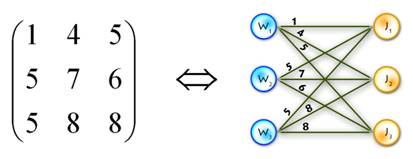
\includegraphics[width=12cm]{grafo.jpg}
        \caption{Planteamiento en forma de grafos del problema de asignación}
    \end{figure}
    \subsection{Algorítmo de solución (Método Húngaro)}
    Existen distintos algorítmos con distintos grados de complejidad computacional que complementan la ressolución de este problema para casos muy particulares, pero el que satisface a grandes rasgos los criterios iniciales y el objetivo a llegar es el
    \emph{Método Húngaro}. Se le denomina como tál gracias a que los primeros aportes al método fueron de Dénes König y Jenő Egerváry, los cuales son dos matemáticos de origen húngaro. \\Cabe destacar los siguientes puntos:
    \begin{itemize}
        \item Está diseñado para resolver \emph{problemas de minimización unicamente}.
        \item El método \emph{trabaja sobre una matriz cuadrada de costos} (\(n\times m=n^2\)).
    \end{itemize}
    \begin{figure}[H]
          \begin{algorithm}[H]
            \SetAlgoLined
            \SetKwProg{Fx}{Function}{:}{end}
            \KwData{la matríz cuadrada ó la tabla cuadrada de costos (\(A_{n\times n}\))}
            \KwResult{el costo total minimizado de dicha matríz ó tabla (\(Z\))}
            \textbf{begin\\}
            Identificar \emph{el mínimo de cada renglón y restarlo a todos los elementos del renglón}\\
            \While{\(i<n+1\)}{
                \(\text{Renglón}_i=\text{Renglón}_i-Min\left(\text{Renglón}_i\right)\)\;
                \(i++\)\;
            }
            Con la matríz resultante del paso anterior, identificar el \emph{el mínimo de cada colúmna y restarlo de todos los elementos de la colúmna}\\
            \While{\(j<n+1\)}{
                \(\text{Colúmna}_j=\text{Colúmna}_j-Min\left(\text{Colúmna}_j\right)\)\;
                \(j++;\)\;
            }
            \Fx{Trazado de lineas(\(n\))}{
                Trazar la \emph{menor cantidad de combinaciones de líneas horizontales y verticales} para cubrir todos los ceros de la matríz reducida\;
                \uIf{\(\#_\text{líneas}=n\)}{
                    Obtener \(Z\) en base a lo encontrado\;
                    \KwRet{\(Z\)}\;
                }
                \uElseIf{\(\#_\text{líneas}<n\)}{
                    Obtener el valor menor de aquellos valores que no se encuentran cubiertos por las lineas\;
                    Restar el valor anterior a los elementos no cubiertos por las lineas\;
                    Sumar dicho valor menor a auellos que se encuentren \emph{en las intersecciones de las lineas horizontales y verticales}\;
                    \KwRet{\emph{Trazado de lineas(\(n\))}}\;
                }
            }
        \end{algorithm}
        \caption{Pseudocódigo del Método Húngaro}
    \end{figure}
    \section{Práctica}
    \subsection{Problema}
    La compañía de manufactura «Jiménez y Asociados» desea realizar una jornada de mantenimiento preventivo a sus tres máquinas principales A, B y C. El tiempo que demanda realizar 
    el mantenimiento de cada máquina es de 1 día, sin embargo la jornada de mantenimiento no puede durar más de un día, teniendo en cuenta que la compañía cuenta con tres proveedores de servicios de mantenimiento debe de
    asignarse un equipo de mantenimiento a cada máquina para poder cumplir con la realización del mantenimiento preventivo. Teniendo en cuenta que según el grado de especialización de cada equipo prestador de servicios de mantenimiento el costo de la tarea varía para cada máquina en particular, 
    debe de asignarse el equipo correcto a la máquina indicada con el objetivo de minimizar el costo total de la jornada. Los costos asociados se pueden observar en la siguiente matríz:
    \begin{figure}[H]
        \centering
        Máquinas
        \[\text{Equipos}\begin{pmatrix}
             &1&2&3\\
            1&\$10&\$9&\$5\\
            2&\$9&\$8&\$3\\
            3&\$6&\$4&\$7
        \end{pmatrix}\]
        \caption{Matríz del problema de asignación de ``Jiménez y Asociados''.}
        \label{fig:matrixprob}
    \end{figure}
    \subsection{Solución}
    \justify
    \textbf{1. Encontrar el valor menor de cada fila:}
    \begin{figure}[H]
        \centering
        Mínimos de cada fila
        \[\begin{pmatrix}
            5\\
            3\\
            4
        \end{pmatrix}\]
        \caption{Mínimos de cada fila de la figura \ref{fig:matrixprob}.}
        \label{fig:minsf}
    \end{figure}
    \justify
    \textbf{2. Construir una nueva matríz con la diferencias entre los valores de la figura \ref{fig:matrixprob} y la figura \ref{fig:minsf}:}
    \begin{figure}[H]
        \centering
        Máquinas
        \[\text{Equipos}\begin{pmatrix}
             &1&2&3\\
            1&10-5=5&9-5=4&5-5=0\\
            2&9-3=6&8-3=5&3-3=0\\
            3&6-4=2&4-4=0&7-4=3
        \end{pmatrix}\]
        \caption{Matríz de diferencias del problema de ``Jiménez y Asociados''.}
        \label{fig:matrixdif}
    \end{figure}
    \justify
    \textbf{3. Con los valores calculados para la figura \ref{fig:matrixdif}, obtener los mínimos de cada colúmna:}
    \begin{figure}[H]
        \centering
        Mínimos de cada colúmna
        \[\begin{pmatrix}
            2&0&0
        \end{pmatrix}\]
        \caption{Mínimos de cada colúmna de la figura \ref{fig:matrixdif}.}
        \label{fig:minsc}
    \end{figure}
    \justify
    \textbf{4. Construir una nueva matríz con la diferencias entre los valores de la figura \ref{fig:matrixdif} y la figura \ref{fig:minsc}:}
    \begin{figure}[H]
        \centering
        Máquinas
        \[\text{Equipos}\begin{pmatrix}
             &1&2&3\\
            1&5-2=3&4-0=4&0-0=0\\
            2&6-2=4&5-0=5&0-0=0\\
            3&2-2=0&0-0=0&3-0=3
        \end{pmatrix}\]
        \caption{Segunda matríz de diferencias del problema de ``Jiménez y Asociados''.}
        \label{fig:matrixdif1}
    \end{figure}
    \justify
    \textbf{5. Trazar la menor cantidad de combinaciones de lineas horizontales y verticales con el objetivo de cubrir todos los ceros de la figura \ref{fig:matrixdif1}:}
    \begin{figure}[H]
        \centering
        Máquinas
        \[\text{Equipos}\begin{pmatrix}
            & & &\tikzmarkV{topA}{}\\ 
            &1&2&3\\
            1&3&4&0\\
            2&4&5&0\\
            \tikzmarkV{StartA}{3}&0&0&\tikzmarkV{EndA}{3}\\
             & & &\tikzmarkV{bottomA}{}
        \end{pmatrix}\]
        \caption{Matríz rayada a partir de la figura \ref{fig:matrixdif1}.}
        \label{fig:matrixlines}
    \end{figure}
    \DrawLineV[red, thick]{topA}{bottomA}
    \DrawLineH[red, thick]{StartA}{EndA}
    Debido a que el número de lineas verticales y/u horizontales necesarias es menor que el número de filas o colúmnas, se realiza el siguiente paso.\\\newline
    \textbf{6. Seleccionar el elemento menor de los valores no-subrayados:}
    \[\text{Elemento menor}_{\text{no-subrayados}}=3\]
    \justify
    \textbf{7. Restar el elemento menor a los valores-no subrayados y adicionar dicho elemento a la intersección  de las lineas:}
    \begin{figure}[H]
        \centering
        Máquinas
        \[\text{Equipos}\begin{pmatrix}
             &1&2&3\\
            1&3-3=0&4-3=1&0\\
            2&4-3=1&5-3=2&0\\
            3&0&0&3+3=6
        \end{pmatrix}\]
        \caption{Matríz modificada a partir de la figura \ref{fig:matrixlines}.}
        \label{fig:matrixpm}
    \end{figure}
    \justify
    \textbf{8. Realizar el paso 5 en la matríz de la figura \ref{fig:matrixpm}:}
    \begin{figure}[H]
        \centering
        Máquinas
        \[\text{Equipos}\begin{pmatrix}
            &\tikzmarkV{topA11}{}& &\tikzmarkV{topA111}{}\\ 
            &1&2&3\\
            1&0&1&0\\
            2&1&2&0\\
            \tikzmarkV{StartA11}{3}&0&0&\tikzmarkV{EndA11}{6}\\
            &\tikzmarkV{bottomA11}{}& &\tikzmarkV{bottomA111}{}
        \end{pmatrix}\]
        \caption{Matríz rayada a partir de la figura \ref{fig:matrixpm}.}
        \label{fig:matrixlines1}
    \end{figure}
    \justify
    \textbf{9. Identificar la biyección (relación 1:1) de los equipos y las máquinas:}
    \begin{figure}[H]
        \centering
        Máquinas
        \[\text{Equipos}\begin{pmatrix}
             &1&2&3\\
            1&\fbox{0}&1&0\\
            2&1&2&\fbox{0}\\
            3&0&\fbox{0}&6
        \end{pmatrix}\]
        \caption{Matríz de biyecciones a partir de la figura \ref{fig:matrixlines1}.}
        \label{fig:matrixbiy}
    \end{figure}
    \justify
    \textbf{10. Obtener el valor de costo mínimo en base al valor encontrado en la figura \ref{fig:matrixprob} a partir de la posición de las biyecciones de la figura \ref{fig:matrixbiy}:}
    \begin{figure}[H]
        \centering
        \[\begin{matrix}
            &\text{Máquinas}& & &\text{Máquinas}\\
            \text{Equipos}\!&\begin{pmatrix}
                &1&2&3\\
               1&\fbox{0}&1&0\\
               2&1&2&\fbox{0}\\
               3&0&\fbox{0}&6
           \end{pmatrix}&:&\text{Equipos}\!&\begin{pmatrix}
            &1&2&3\\
           1&\fbox{\$10}&\$9&\$5\\
           2&\$9&\$8&\fbox{\$3}\\
           3&\$6&\fbox{\$4}&\$7
       \end{pmatrix}\therefore
        \end{matrix}\]
        \caption{Biyección de la figura \ref{fig:matrixpm} con la figura \ref{fig:matrixbiy}.}
        \label{fig:relationbiy}
    \end{figure}
    \[\therefore\begin{matrix}
        Z&=\left(\text{Equipos}_1\cap \text{Máquinas}_1 \right)+ \left(\text{Equipos}_2\cap \text{Máquinas}_3\right) + \left(\text{Equipos}_3\cap \text{Máquinas}_2\right)&\\
         &=10+4+3&\\
         &=17&
    \end{matrix}\]
    Dando por concluido el problema.

    \DrawLineV[red, thick]{topA11}{bottomA11}
    \DrawLineH[red, thick]{StartA11}{EndA11}
    \DrawLineV[red, thick]{topA111}{bottomA111}

    \section{Conclusión}
    El problema de asignación y su resolución por el algoritmo descrito nos permiten plantear de otra manera los incovenientes acorde a los detalles de optimización 
    deseados para costear de una mejor manera los procesos los cuales se desee emplear.

    \newpage
    \lhead{}
    \addcontentsline{toc}{section}{Referencias}
    \printbibliography

\end{document}